\subsection{Konzentrationsänderung von Kaliumhexacyanoferrat(III)}
\authors{David Bürg, Patricia Mühren}

\subsubsection{Durchführung}

Um die Auswirkungen der Konzentration von $\mathrm{K}_3[\mathrm{Fe}(\mathrm{CN})_6]$ auf die Lumineszenz beschreiben zu können, wird die Grundlösung (G2) mit zwei verschiedenen Konzentrationen von $\mathrm{K}_3[\mathrm{Fe}(\mathrm{CN})_6]$ mit der gleichen Vorgehensweise in aufeinanderfolgenden Versuchen angereichert. Die erste Variation ist die G2-Lösung aus 15 ml L2 und 2 ml $\mathrm{H}_2\mathrm{O}_2$ ($\mathrm{G}2^-$), die andere eine G2-Lösung aus 60 mL L2 und 2 ml $\mathrm{H}_2\mathrm{O}_2$ ($\mathrm{G}2^+$). Zu den Grundlösungen wird dann demineralisiertes Wasser hinzugegeben, damit später wieder die 250-ml-Marke erreicht wird.
Dieser Versuch wird mit beiden Grundlösungen ($\mathrm{G}2^-$) und $\mathrm{G}2^+$), wie zuvor beschrieben, durchgeführt. Nach dem Zusammenschütten von G1 und G2 werden in konstanten Zeitintervallen Aufnahmen getätigt.
 
\subsubsection{Beobachtungen}

Bei der Zusammengabe von G1 und $\mathrm{G}2^-$ beobachtet man eine Emission von blauem beziehungsweise türkisem Licht.
Aus den Aufnahmen [Abb. \ref{dsafigure:beispiel1}] geht hervor, dass mit fortschreitender Zeit die Intensität des emittierten Lichtes abnimmt. Vergleicht man die vorher genannten Aufnahmen mit den Aufnahmen von $\mathrm{G}2^+$, so kann man feststellen, dass die Intensität des emittierten Lichtes bei $\mathrm{G}2^+$ höher ist als bei allen Aufnahmen von $\mathrm{G}2^-$. Diese Beobachtung wird auch mit technisch ermittelten  Werten durch ImageJ \cite{ImageJ}, siehe Tabelle \ref{dsatable:beispiel0}, belegt. Bei der Ermittlung der Intensität wird über den Grauwert entlang einer rechteckigen Fläche integriert.  

\begin{dsatable}
 \caption{Intensitätswerte des emittierten Lichtes für die einzelnen Aufnahmen von unterschiedlichen          Bechergläsern, einmal mit $\mathrm{G}2^+$ und das andere Mal mit $\mathrm{G}2^-$. Dabei entstehen beim Festhalten der Intensität der Lumineszenz mit der Grundlösung von 15 ml $\mathrm{K}_3[\mathrm{Fe}(\mathrm{CN})_6]$ vier Aufnahmen, mit der Grundlösung von 60 ml $\mathrm{K}_3[\mathrm{Fe}(\mathrm{CN})_6]$ eine Aufnahme.}
 \centering
 \begin{tabular}{lcr}
  \toprule
   Zeit            & Intensitätswert\\
  \midrule
   2 s			   & 58.013\\
   4 s		       & 47.016\\
   6 s		       & 36.886\\
   8 s		       & 28.978\\
  \midrule
   2 s		       & 72.5588\\
  \bottomrule
 \end{tabular}
 \label{dsatable:beispiel0}
\end{dsatable}

\begin{dsafigure}
 \centering
 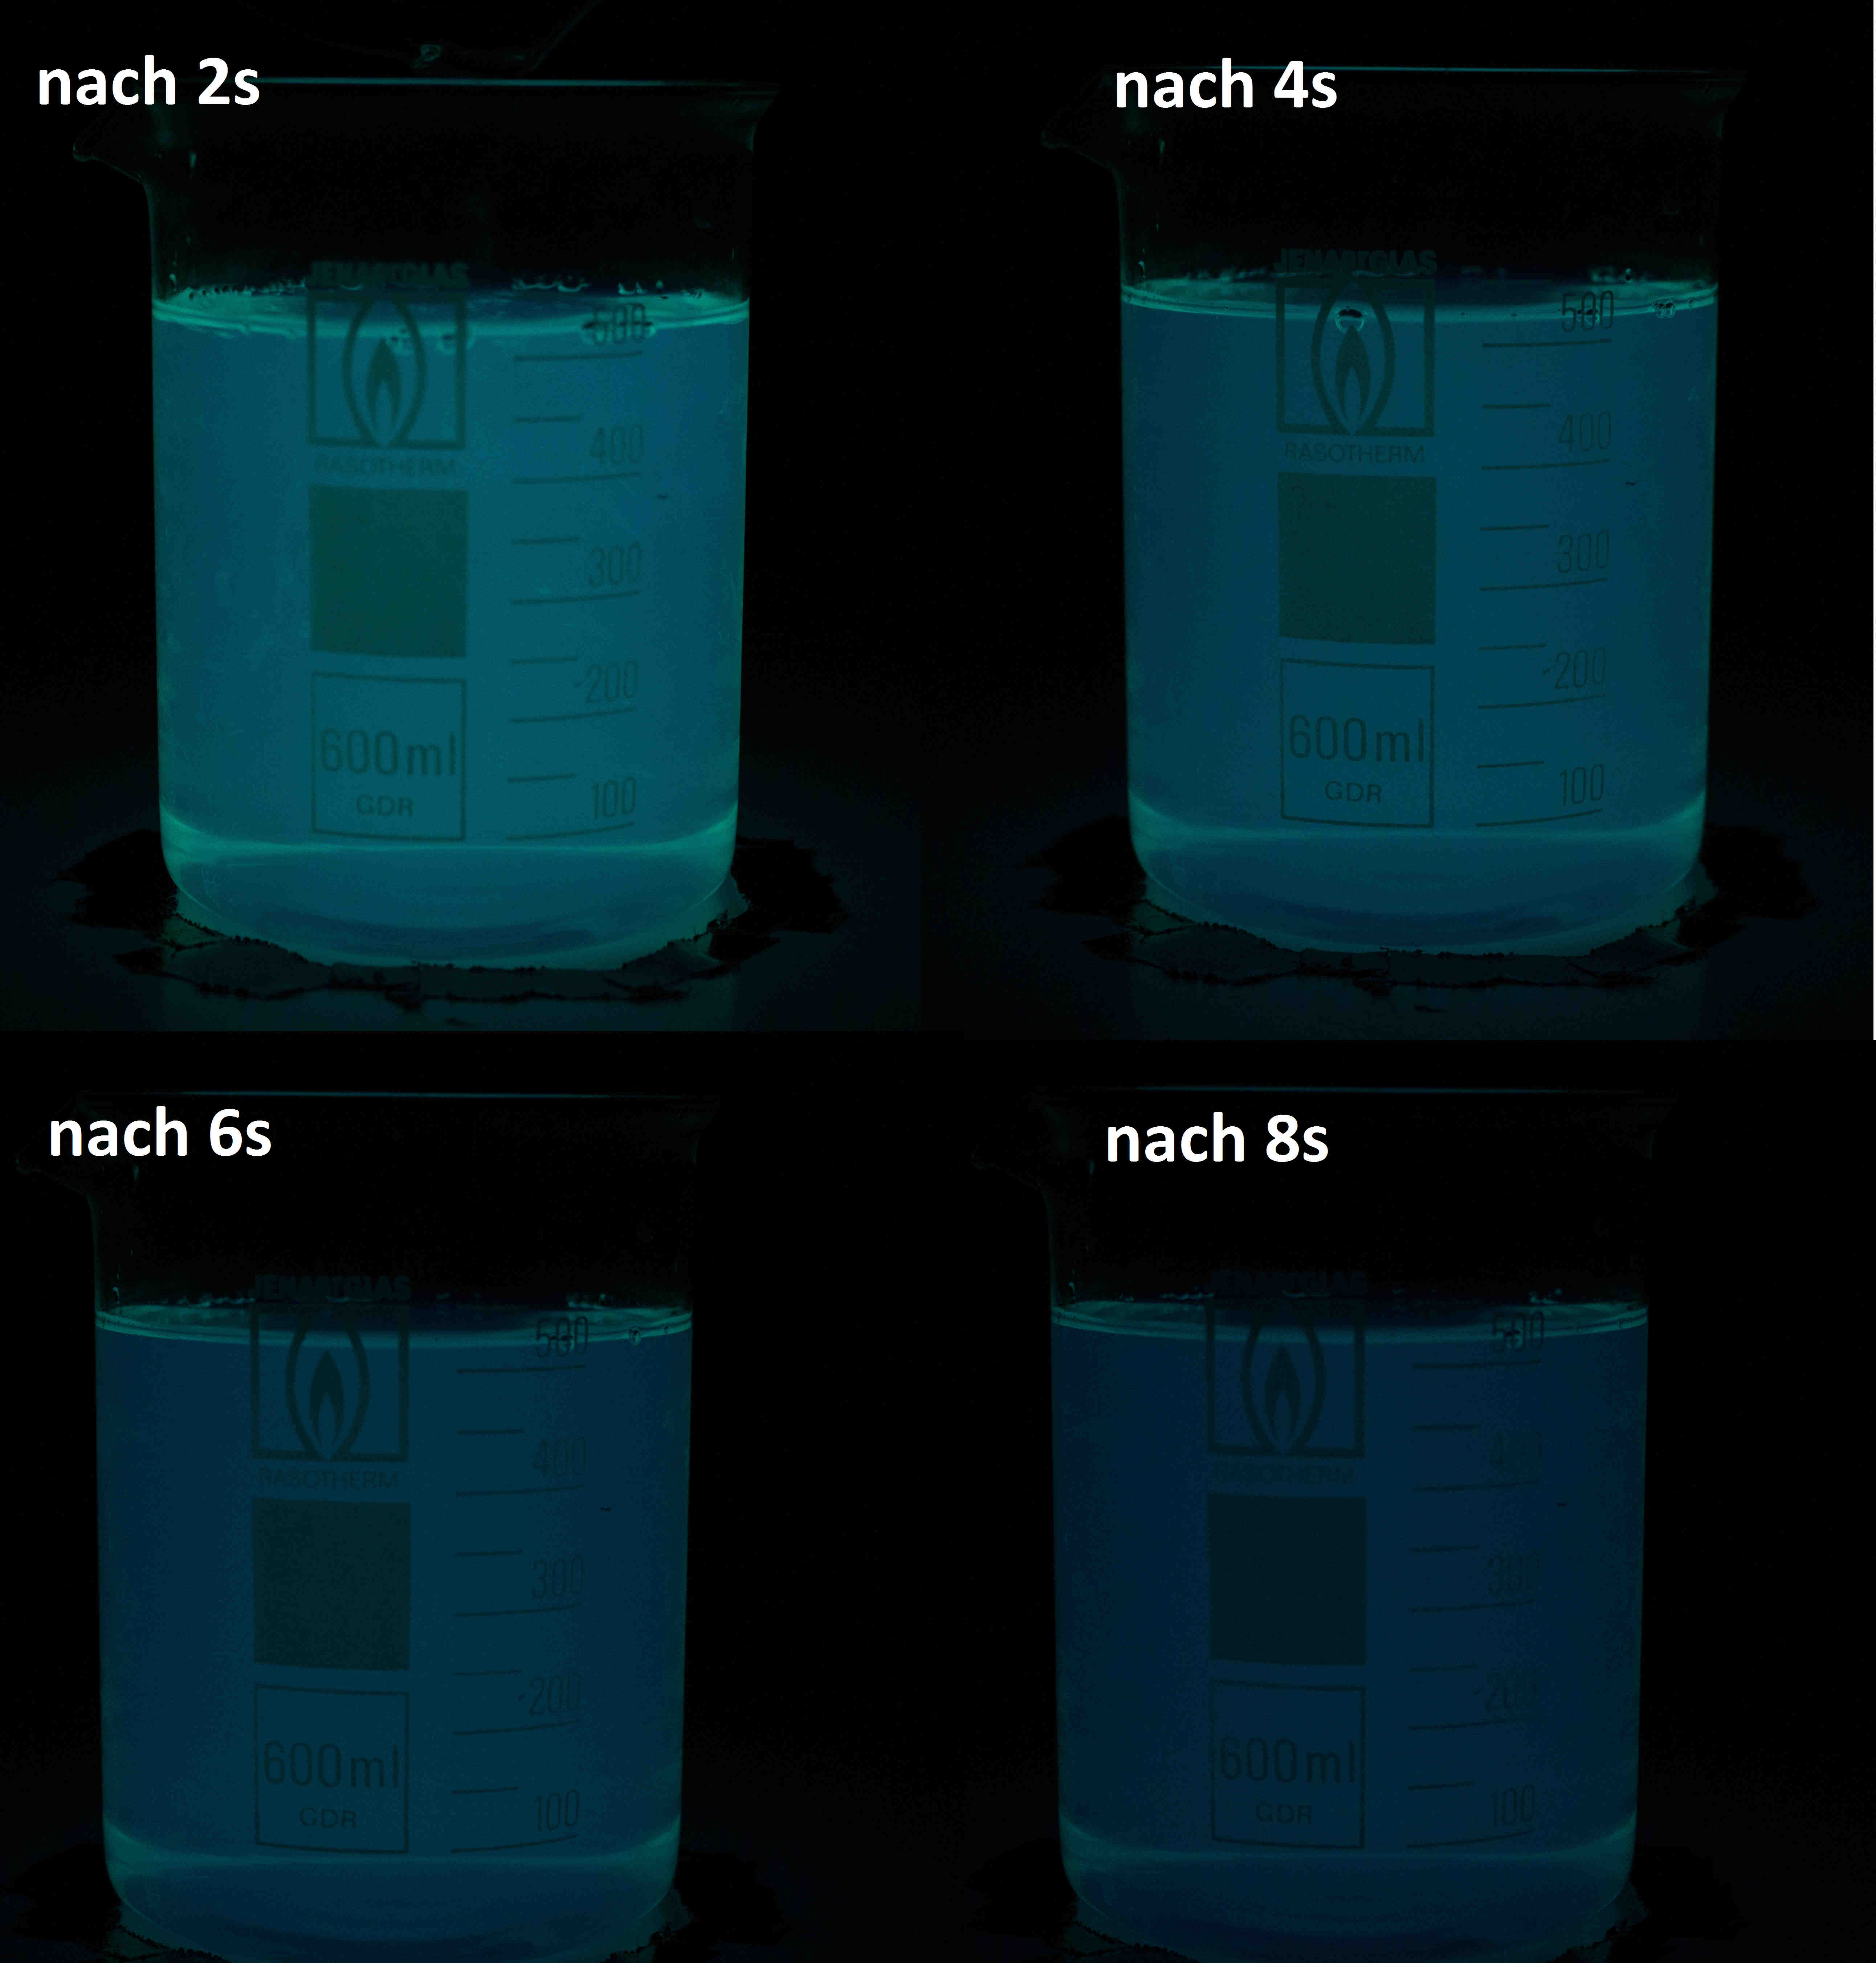
\includegraphics[scale=0.05]{G2minusSeriemitSekunden2.jpg}
 \caption{G1 und $\mathrm{G}2^-$ --> Aufnahme nach zwei, vier, sechs und acht Sekunden}
 \label{dsafigure:beispiel1}
\end{dsafigure} 
